\chapter{ USER STORY}


\section{Page d'authentification}
Les captures d'écran ci-dessous montrent l'interface graphique intuitive et facile à utiliser que nous avons mise en place. Au lancement de l'application, l'utilisateur tombe sur une fenêtre d'authentification où il doit renseigner son numéro de téléphone, son pseudonyme et son mot de passe. Les informations saisies par l'utilisateur sont vérifiées. Le numéro de téléphone ne doit comprendre que 10 caractères qui sont obligatoirement tous des chiffres de 0 à 9. Le pseudo de l'utilisateur est également vérifié, celui-ci ne doit pas comporter de caractère étoile "*" et de plus sa taille ne peut excéder 9 caractères. Une fois ces informations saisies mais aussi vérifiées et que l'utilisateur est authentifié auprès du serveur, cette page ne sera plus affichée, au lancement de l'application l'utilisateur sera directement redirigé vers la page principale de l'application. 
    \begin{figure}[H]
    \begin{center}
    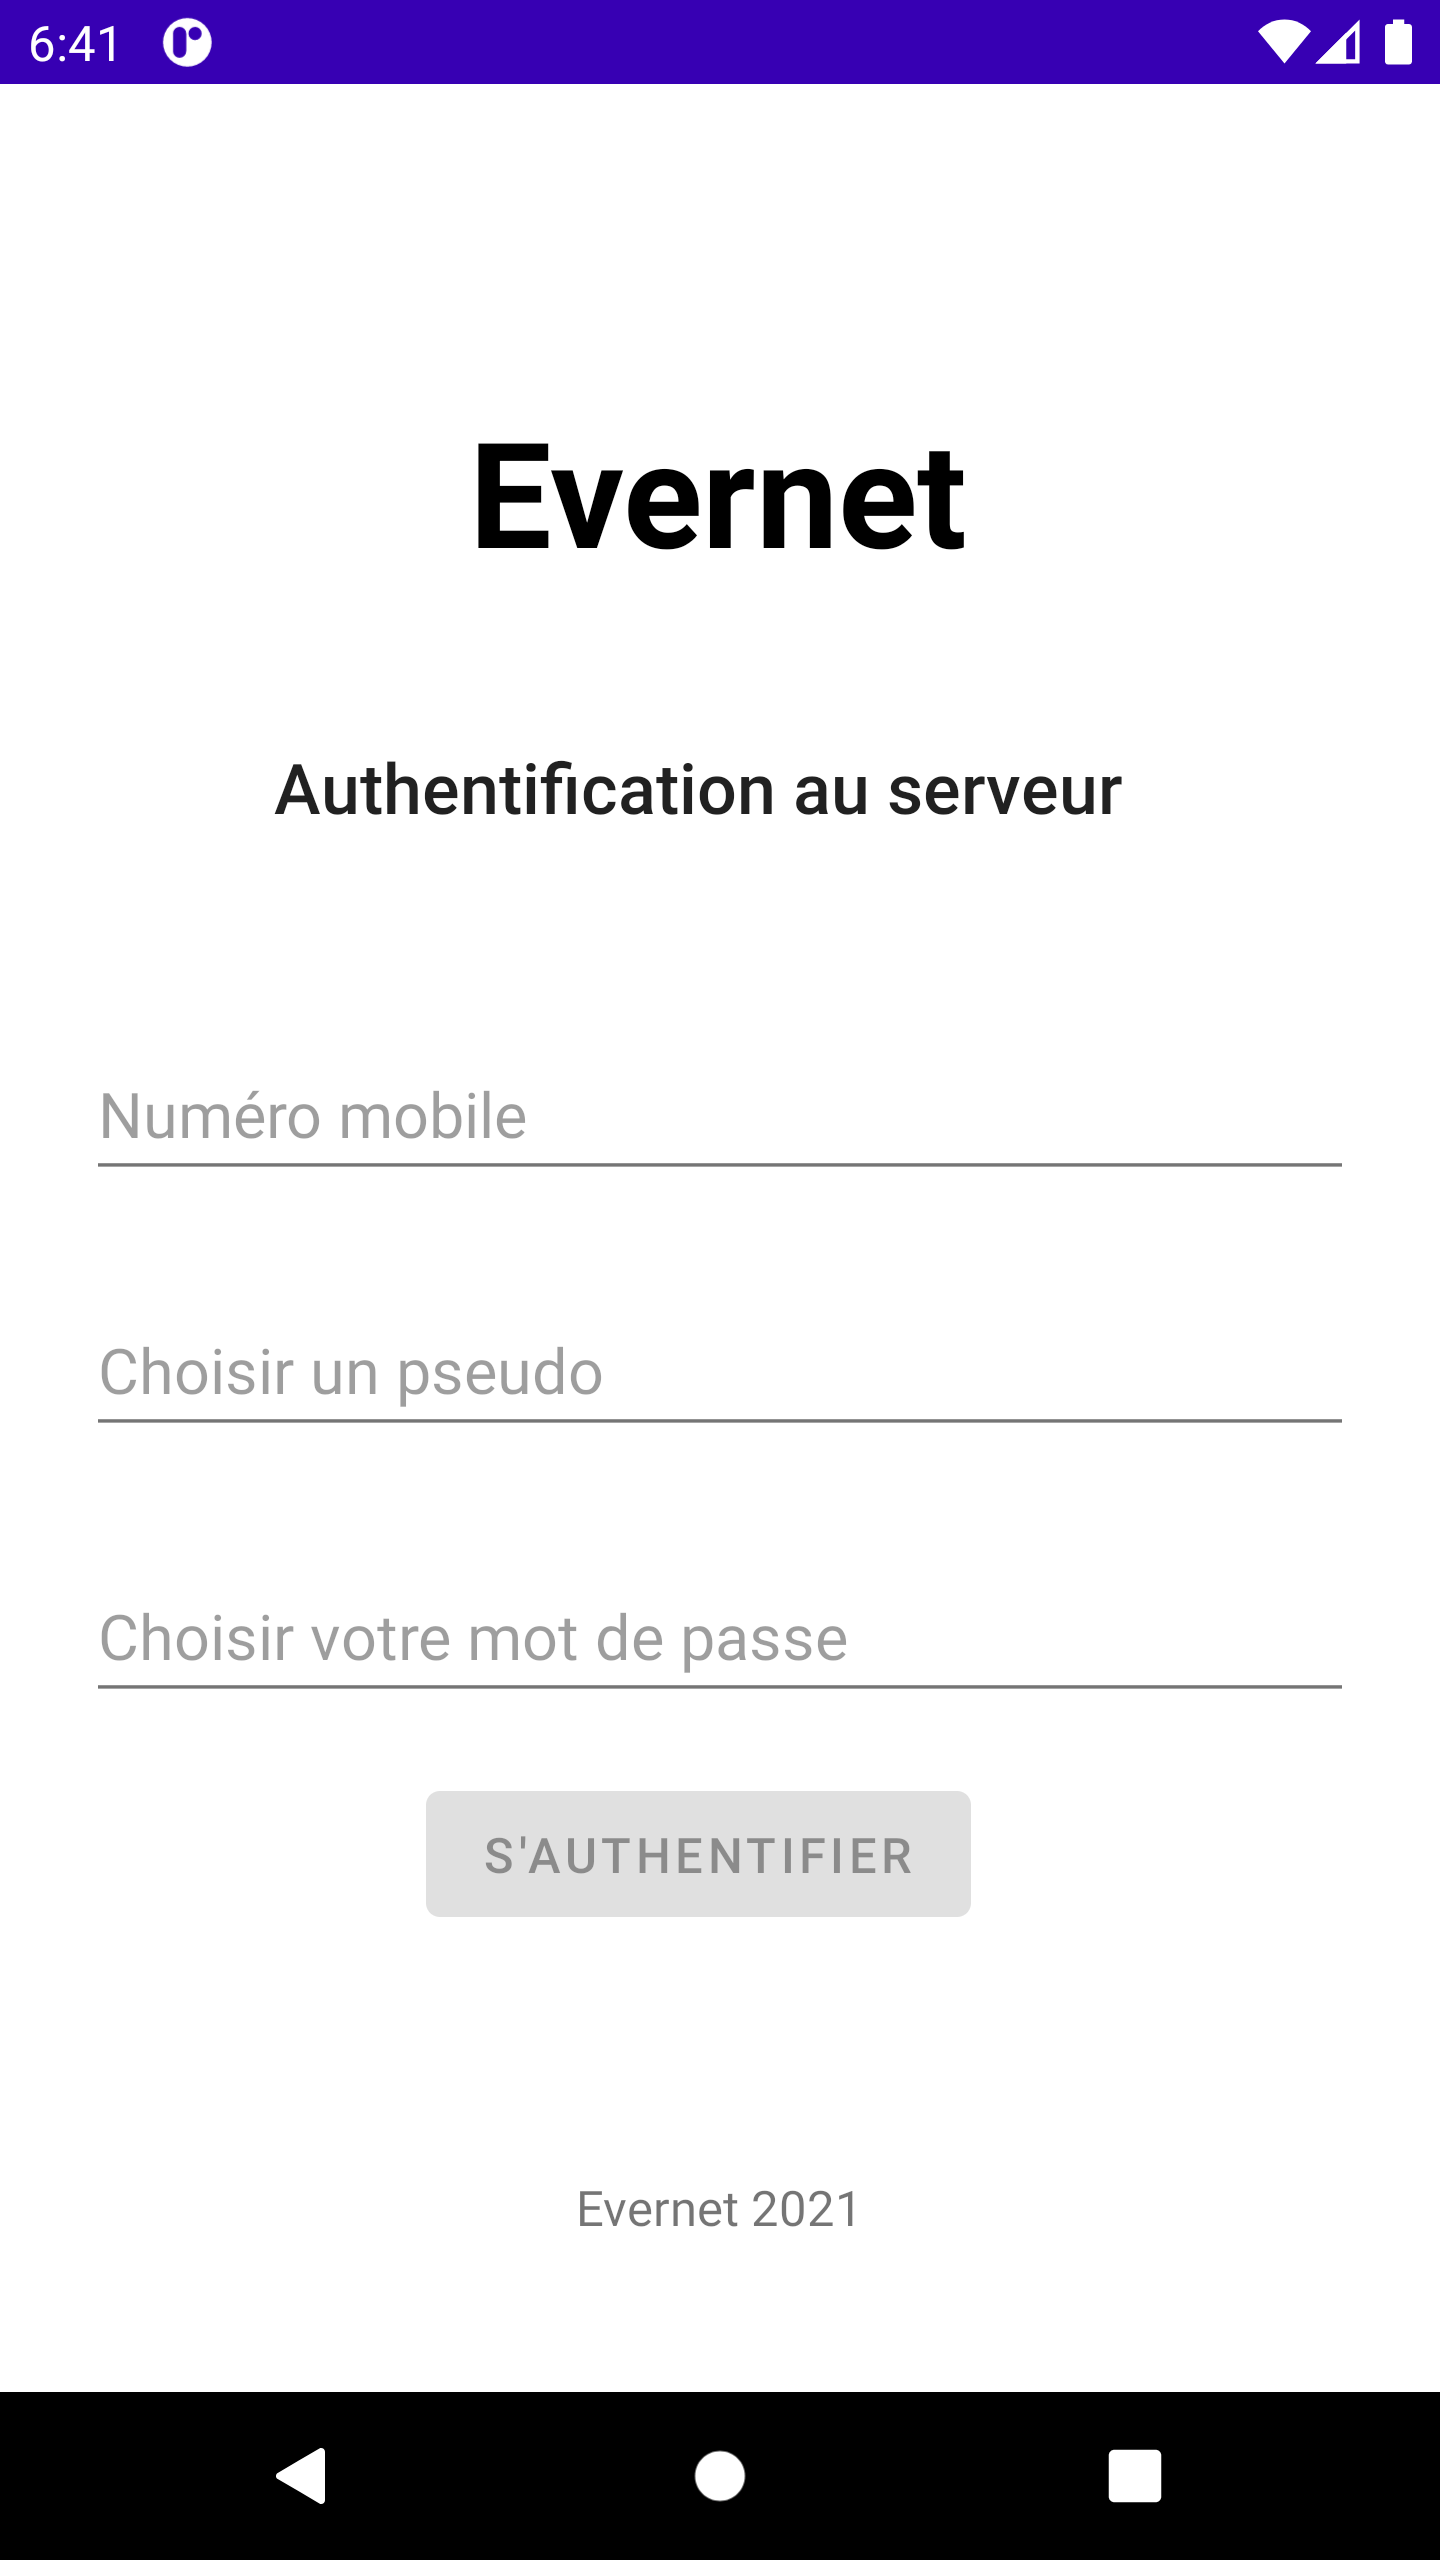
\includegraphics[width=7cm]{images/auth.png}
    \caption{Page d'authentification de l'application.}
    \end{center}
    \end{figure}
    
\section{Page principale}    
Après l'authentification, l'utilisateur arrive sur la page principale de l'application. Celle-ci comporte trois boutons, celui pour aller dans la page d'ajout des contacts, celui pour accéder au menu permettant l'envoi d'une image, ainsi qu'un bouton pour quitter l'application. Par défaut le menu permettant l'envoi d'une image est directement affiché. Celui-ci offre à l'utilisateur la possibilité de choisir une image à envoyer dans sa galerie, de choisir un destinataire parmi sa liste de contact et d'envoyer une image. Une fois l'image à envoyer sélectionnée, celle-ci apparaît dans le cadre d'image encore vide au lancement de l'application.
 
    \begin{figure}[H]
    \begin{center}
    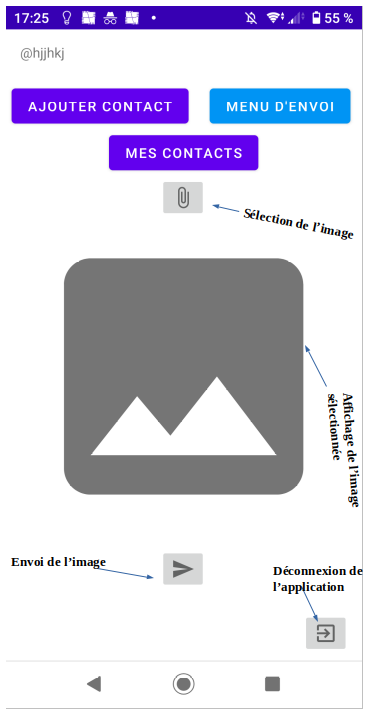
\includegraphics[width=7cm]{images/send_picture.png}
    \caption{Page d'accueil de l'application.}
    \end{center}
    \end{figure}
    

En appuyant sur le bouton "Mes contacts", l'utilisateur va voir apparaître une nouvelle page regroupant l'ensemble des contacts enregistrés sur l'application. Ceux-ci sont affichés sous forme de liste comportant le pseudo de l'utilisateur et en dessous de celui-ci l'id associé a cet utilisateur précédé d'un '\#'.    
\begin{figure}[H]
    \begin{center}
    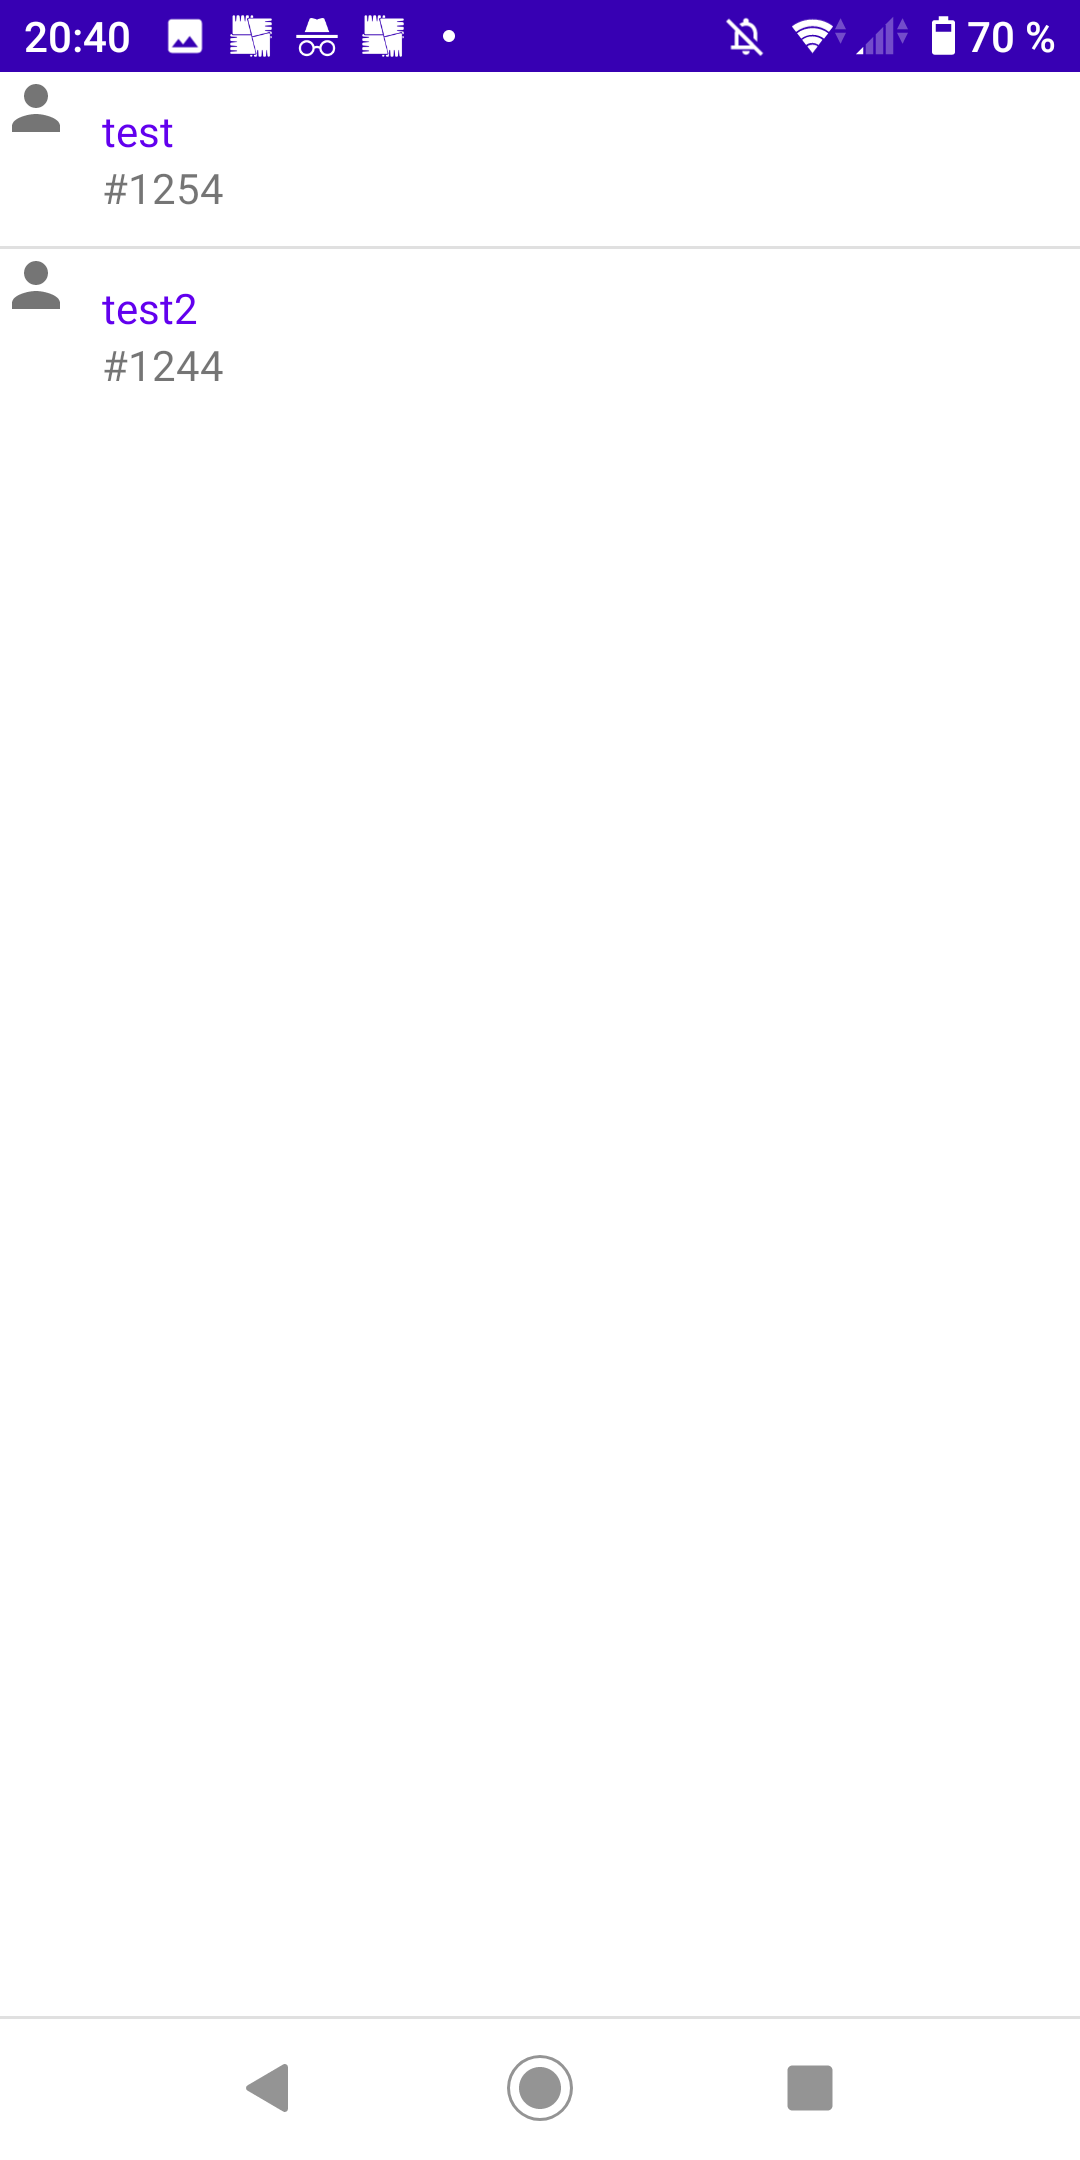
\includegraphics[width=5cm]{images/Contact_Page.png}
    \caption{Liste de Contacts.}
    \end{center}
    \end{figure}
    
Le menu permettant l'ajout de contact est accessible depuis la page principale par l'intermédiaire du bouton "Ajouter contact". Ce menu permet à l'utilisateur de saisir dans deux champs, le nom du contact qu'il souhaite ajouter ainsi que son id. Le bouton "sauvegarder" permet de sauvegarder ce contact dans une base sous forme de fichiers texte (.txt). Ce fichier permet de sauvegarder les contacts enregistrés dans l'application de manière permanente ainsi lorsque l'utilisateur quitte l'application ses contacts préférés ne sont pas effacés.
    \begin{figure}[H]
    \begin{center}
    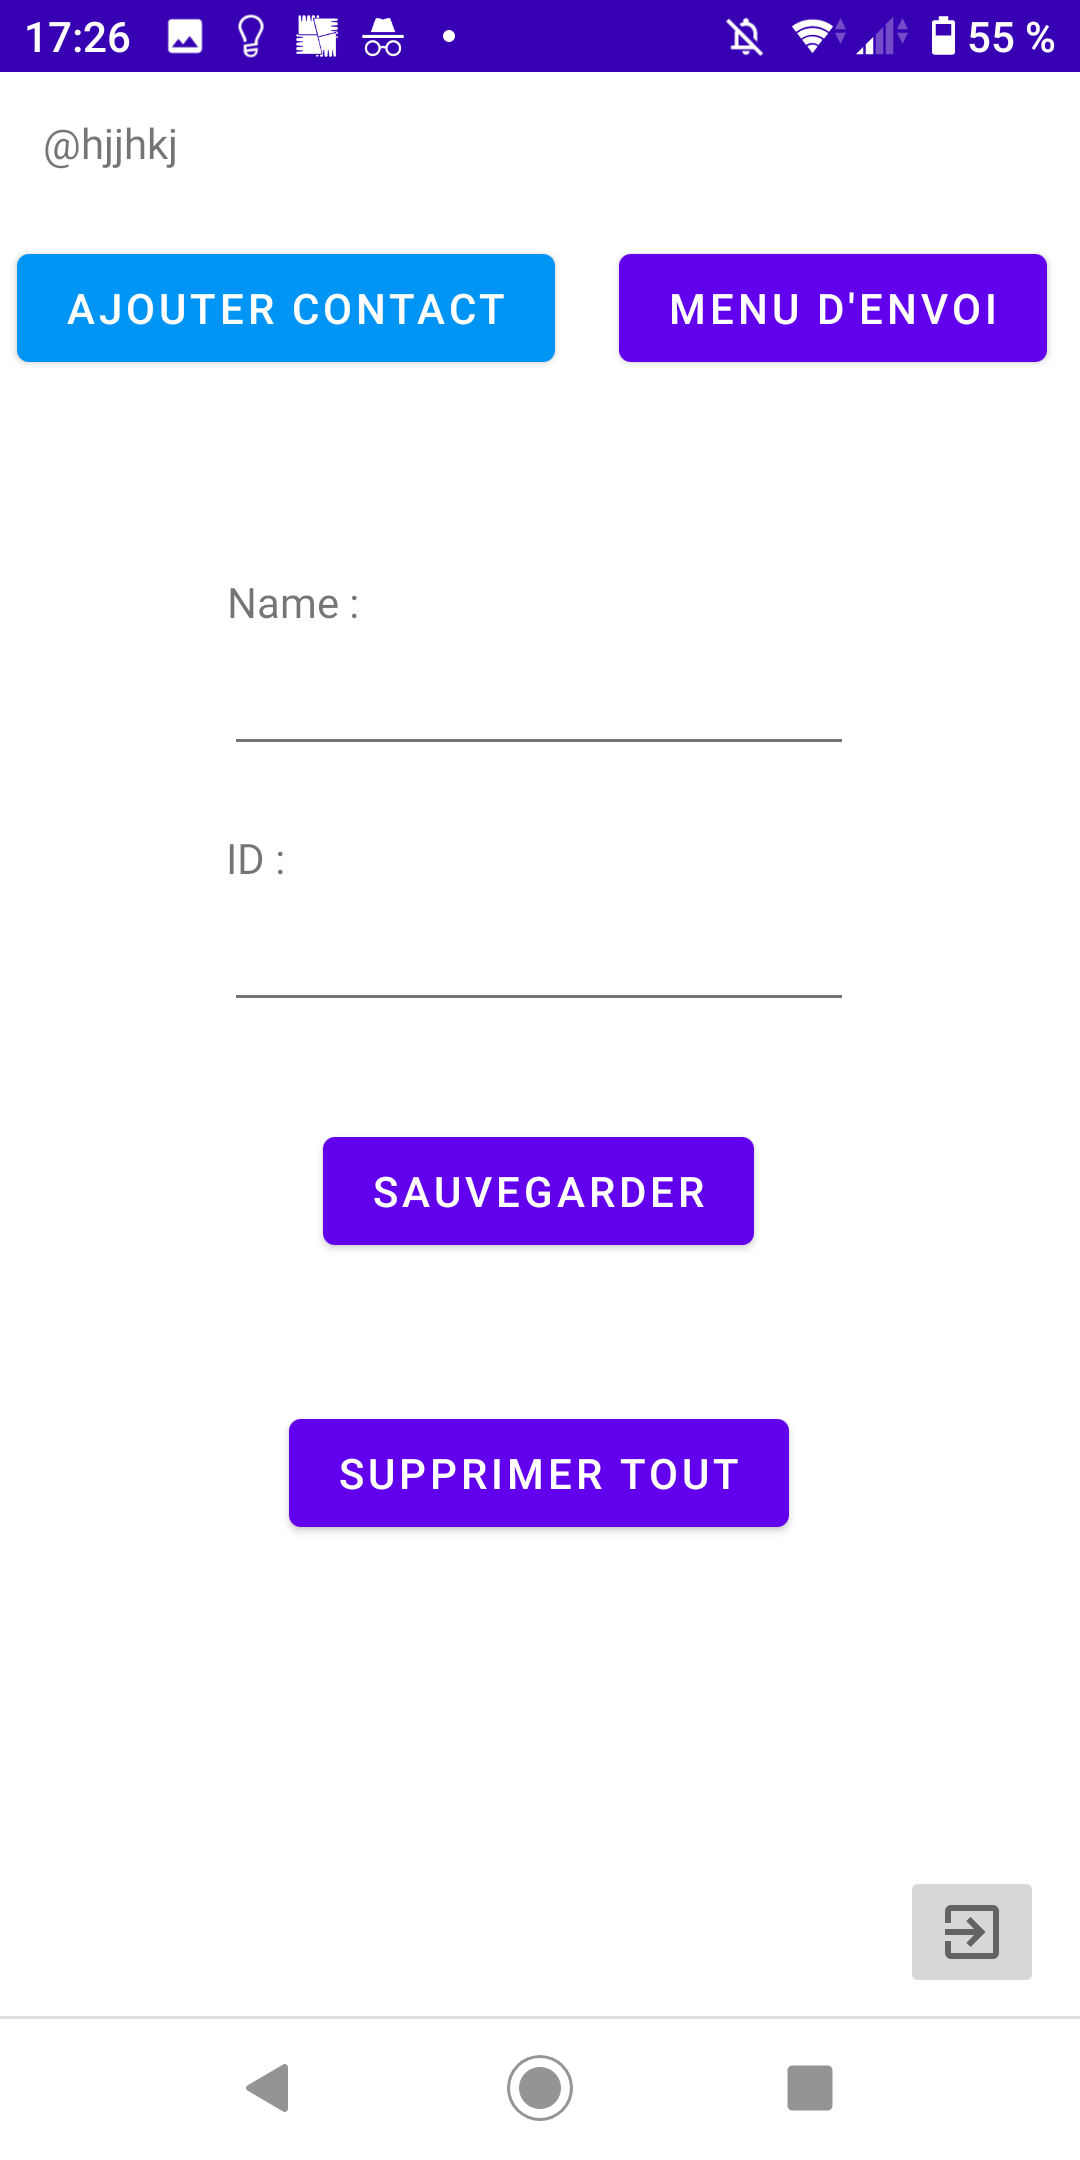
\includegraphics[width=7cm]{images/add_contact.png}
    \caption{Ajouter un Contact.}
    \end{center}
    \end{figure}
        